\chapterimage{./Pictures/cover-socket} % Chapter heading image
\chapter{TP7+TP8 : Communication socket}

\section{Communication distante en utilisant l’outil netcat}

\subsection{Exercice 1 : Découverte de la commande nc : netcat}
\textit{L’objectif de cet exercice est de nous familiariser avec une commande puissante appelée \mintinline{shell}{nc}. Cette commande, inspirée de la commande \mintinline{shell}{cat}, permet d’afficher et de recevoir un flux d’octets, non pas à l’écran et depuis le clavier, mais sur ou depuis le réseau, et plus précisément vers un processus distant identifié par une adresse ip un numéro de port et un mode (connecté "TCP" ou non connecté "UDP")}

Afin de lancer un serveur TCP sur le port 3000 nous utilisons la commande \mintinline{shell}{nc -l 3000}. Elle affichera à l'écran tous les messages recu par le serveur.
Afin de lancer un client TCP qui se connectera au serveur TCP nous utilisons la commande \mintinline{shell}{nc localhost 3000}

\subsection{Exercice 2 : Utilisation de la commande nc : netcat pour le transfert de fichier et l’évaluation de la bande passante}
\textit{La commande netcat, souvent réduite au nom nc, est un utilitaire très puissant qui reprend le principe de la commande cat sur un support réseau. Les possibilités de cette commande sont énormes, et permettent de mettre en place très simplement un serveur en mode connecté ou non connecté pour transférer du texte ou un fichier. Cette commande peut également jouer le rôle de client.}

Pour transférer un fichier il faut :
\begin{itemize}
  \item Coté émetteur : utiliser la commande \mintinline{shell}{nc <ip_address>:<port> > <filename>}
  \item Coté récepteur : utiliser la commande \mintinline{shell}{nc <ip_address>:<port> < <filename>}
\end{itemize}

La commande \mintinline{shell}{time} mise avant \mintinline{shell}{nc} nous pouvons avoir les informations de temps de transfert.

\subsection{Exercice 3 : Une histoire de serveurs concurrents ...}
\textit{Dans cet exercice, nous regardons quelles capacités de cohabitation existent entre des serveurs qui voudraient utiliser le même port de communication}

Il est possible de connecter plusieurs serveur tcp.
\begin{itemize}
  \item Le premier hôte se connectera au premier server TCP créé.
  \item Le deuxième hôte se connectera au deuxième server TCP créé.
  \item ainsi de suite.
\end{itemize}
Il en est de même pour la connexion de plusieurs serveurs UDP.

Si nous souhaitons faire un montage avec un serveur tcp et un serveur udp, les clients tcp communiqueraient avec le serveur tcp et les clients udp avec les serveurs udp.
Il s'affichera un message d'erreur sur les serveur TCP \texttt{Address already use}. Cela signifie que si nous nous connectons sur un port avec plusieurs serveurs nous discuterons avec les deux serveurs.

%\subsection{Exercice 4 : Comprendre une requête HTTP}
%\textit{Dans cet exercice, nous regardons une utilisation simple et originale de \mintinline{shell}{netcat} : comprendre ce que votre navigateur internet envoie comme information lorsqu’il effectue une requête sur un site web}

\section{Développement d’un client et d’un serveur en C}
\subsection{Exercice 5 : Mise en place d’une communication en mode non connecte}
\textit{L’objectif de cet exercice est de découvrir les fonctions et structures de base en C permettant une communication en mode non connecté UDP.}

Nous proposerons le code ci-dessous afin d'implementer un client UDP ayant le comportement demandé :
\inputminted[linenos,firstline=31, lastline=87]{cpp}{../sources/cpp/TP7-8/clientUDP.c}

Nous proposerons le code ci-dessous afin d'implementer un serveur UDP ayant le comportement demandé :
\inputminted[linenos,firstline=34, lastline=104]{cpp}{../sources/cpp/TP7-8/serveurUDP.c}

Après avoir lancé le serveur UDP nous testerons la communication entre le serveur UDP et le client UDP à l'aide de la commande \mintinline{bash}{UDClient <IP> <port> <message>} ainsi nous précisons au client l'IP et le port du serveur mais aussi le message que nous souhaitons envoyer.
\mintinline{shell}{0.0.0.0 5000 "tset ysae"}

Le message reviens dans le même ordre \texttt{tset ysae}.

\subsection{Exercice 6 : Création d’une architecture (client UDP) - (relai UDP-TCP) - (serveur TCP)}

\textit{L'objectif de cet exercice est de manipuler les deux mode (connecté et non connecté), en faisant communiquer un serveur tournant en TCP avec un client tournant en UDP. Cette communication n’est pas directement possible et nécessite un processus intermédiaire qui fera le relai entre le client et serveur.}

À l'aide des instructions donné dans le sujet de l'exercice nous pouvons implémenter le code principale d'un serveur TCP étant similaire à celui d'un serveur UDP:
\inputminted[linenos, firstline=34, lastline=104]{cpp}{../sources/cpp/TP7-8/serveurTCP.c}

Nous pouvons ensuite implémenter le le code du relai UDP-TCP :
\inputminted[linenos, firstline=34, lastline=104]{cpp}{../sources/cpp/TP7-8/relaiUDPTCP.c}

Après avoir lancé le serveur TCP ainsi que le relai UDP-TCP nous testerons la communication entre le serveur UDP, le relai UDP TCP et le server TCP à l'aide de la commande \mintinline{bash}{UDPClient <IP> <port> <message>} ainsi nous précisons au client l'IP et le port du serveur mais aussi le message que nous souhaitons envoyer.
\mintinline{shell}{0.0.0.0 5000 "tset ysae"}

Le message reviens dans le même ordre \texttt{easy test}.

\begin{figure}[H]
\centering
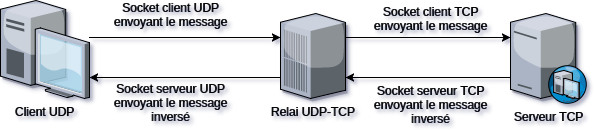
\includegraphics[width=300pt]{./cpp/Pictures/tp7+tp8-relay-UDP-TCP}
\caption{Relai UDP-TCP}
\label{Relai UDP-TCP}
\end{figure}

\section{Exercices bonus}
\subsection{Exercice 7 : Résolution de noms}
\textit{Cet exercice à pour objectif de manipuler la fonction \mintinline{cpp}{gethostbyname()}. Cette fonction permet de transformer des noms de domaines en adresse ip, en interrogeant un serveur DNS.}
Les différents appareils connecté à internet communique entre eux grâce aux adresse IP. Afin d'accéder aux adresse IP depuis un nom de domaine, les appareils demandent à un serveur DNS. DNS signifie système de nom de domaine (Domain Name System en anglais).

On peut facilement prendre pour exemple l'accès à l'adresse \texttt{google.fr} et le schématiser de la manière suivante :

\begin{figure}[H]
\centering
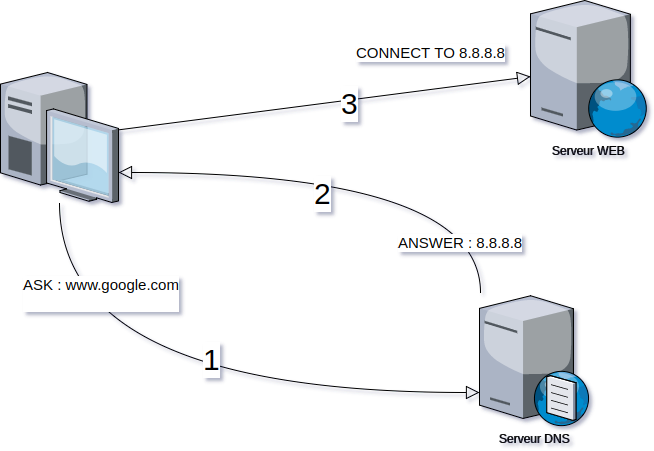
\includegraphics[width=300pt]{./cpp/Pictures/tp7+tp8-DNS}
\caption{Résolution DNS}
\label{Résolution DNS}
\end{figure}

La machine demande au serveur DNS l'adresse IP du domaine \texttt{google.fr} qui lui répond \texttt{8.8.8.8}, ainsi la machine pourra se connecter au serveur à l'adresse indiqué.

À l’aide du manuel et des exemples disponibles sur internet, ainsi que de la documentation de la fonction \mintinline{cpp}{gethostbyname()} permettant la translation d’un nom de domaine vers une adresse IP. J'ai créé un programme qui affiche les adresses IP des noms de domaine "www.yahoo.fr", "www.gmail.com" et "www.u-bourgogne.fr".

\inputminted[linenos,firstline=10, lastline=36]{cpp}{../sources/cpp/TP7-8/getHostByName.c}

%\subsection{Exercice 8 : Serveur multi-client en mode connecté}
